% !TEX program = xelatex
% =============================================================================
%  数字集成电路设计 · 题目一 · 课堂汇报（约 15 分钟 / 24 页）
%  16x16 Transformer 注意力计算模块 —— 定点量化 + 行融合
%
%  编译：pwsh -File .\build.ps1 -Name ic_slides -Open
%  数字口径：docs/engineering/05（SMIC40 九角）、docs/theory/01（位宽）
%
%  排版约定：表格单元格一律只放单行文字（beamer 下 p{} 定宽列的中文折行会压行），
%            需要折行的说明改写为段落或 \parbox。
% =============================================================================
\documentclass[10pt,aspectratio=43,mathserif]{beamer}

%%%%-----导入宏包-----%%%%
\usepackage{seu}
\usepackage{xeCJK}
\usepackage{amsmath,amsfonts,amssymb,bm}
\usepackage{color}
\usepackage{graphicx,hyperref,url}
\usepackage{booktabs,array,multirow}
\usepackage{tikz}
\usetikzlibrary{positioning,arrows.meta,calc,decorations.pathreplacing}
%%%%%%%%%%%%%%%%%%

%%%%-----设置字体-----%%%%
\setsansfont[Path=fonts/]{Helvetica}
\setCJKmainfont[Path=C:/Windows/Fonts/,BoldFont=simhei.ttf,ItalicFont=simkai.ttf]{simsun.ttc}
\setCJKsansfont[Path=C:/Windows/Fonts/,BoldFont=msyhbd.ttc,AutoFakeBold=2]{msyh.ttc}
\setCJKmonofont[Path=C:/Windows/Fonts/]{simfang.ttf}
% ①②③④ 属 Enclosed Alphanumerics，默认会被分给 Helvetica 而缺字，强制归 CJK
\xeCJKDeclareCharClass{CJK}{"2460 -> "2473}

\definecolor{cR}{RGB}{108,104,94}
\definecolor{cA}{RGB}{40,84,120}
\definecolor{cB}{RGB}{46,104,72}
\definecolor{cS}{RGB}{186,118,36}
\definecolor{cW}{RGB}{150,60,48}

\tikzset{
  blk/.style={draw=black!40,fill=white,rounded corners=1.2pt,align=center,inner sep=3pt},
  hdr/.style={draw=black!40,fill=black!7,rounded corners=1.2pt,align=center,inner sep=3pt},
  acc/.style={draw=cA!60,fill=cA!9,rounded corners=1.2pt,align=center,inner sep=3pt},
  grn/.style={draw=cB!60,fill=cB!9,rounded corners=1.2pt,align=center,inner sep=3pt},
  arr/.style={-{Latex[length=1.7mm]},draw=black!55,thick},
  lab/.style={font=\scriptsize,inner sep=2pt},
}

% adjustbox 依赖 xkeyval/adjcalc，本机 TeX 未装；用 graphicx 自带 resizebox 手写
% 「超过版心宽才缩放」的盒子，避免为此再装三个宏包
\makeatletter
\newsavebox{\fitbox@b}
\newcommand{\fitbox}[1]{%
  \sbox{\fitbox@b}{#1}%
  \ifdim\wd\fitbox@b>\linewidth
    \resizebox{\linewidth}{!}{\usebox{\fitbox@b}}%
  \else
    \usebox{\fitbox@b}%
  \fi}
\makeatother

\beamertemplateballitem

%%%%----首页信息----%%%%
\title[16$\times$16 注意力模块]{16$\times$16 Transformer 注意力模块\\[0.5mm]的定点化与行融合实现}
\subtitle{\fontsize{9pt}{13pt}\selectfont \textbf{数字集成电路设计 · 2026 秋 · 题目一}}
\author[汪涵\quad 黄昌文\quad 许心怡\quad 郭丰硕]{汪涵\quad 黄昌文\quad 许心怡\quad 郭丰硕}
\institute[SEU]{东南大学 \; 集成电路学院}
\date[2026.11]{2026 年 11 月}

\begin{document}

%%%% ============ 封面 ============
\begin{frame}
\titlepage
\end{frame}

%%%% ============ 目录 ============
\begin{frame}
\frametitle{\textbf{目录}}
\textbf{\tableofcontents}
\end{frame}

%%%% ============ 1 分工 ============
\section[分工]{团队分工}

\begin{frame}[t]
\frametitle{\textbf{四个工作包：一条依赖链，不是四份独立的活}}
\footnotesize
\begin{center}
\fitbox{%
\begin{tabular}{lcl}
  \toprule
  工作包 & 负责人 \quad 学号 & 职责与交付物 \\
  \midrule
  P1 \; 算法与数值 & 汪涵 \quad 266900 &
    \shortstack[l]{架构对比 \;·\; $QK^{\top}$／$PV$ \;·\; Softmax \;·\; 位宽与舍入\\
                   模型数值契约 \;·\; 引用更正}\\[1.2mm]
  P2 \; 集成与流水 & 黄昌文 \quad 266909 &
    \shortstack[l]{顶层 FSM \;·\; 行融合 \;·\; A／B／C 三级 \;·\; erow bank\\
                   B--C 反压 \;·\; 流式输出}\\[1.2mm]
  P3 \; 验证与复现 & 许心怡 \quad 269873 &
    \shortstack[l]{六类激励 \;·\; reset／cont \;·\; 向量独立性 \;·\; Table~1 原料\\
                   回归／哈希／manifest}\\[1.2mm]
  P4 \; PPA 与报告 & 郭丰硕 \quad 266617 &
    \shortstack[l]{$D$／$E$ 口径 \;·\; 综合／功耗／P\&R \;·\; Table~2／3\\
                   claim ledger \;·\; PPT／贡献表 \;·\; TA}\\
  \bottomrule
\end{tabular}}
\end{center}
\vspace{0.5mm}
\begin{center}
\begin{tikzpicture}[node distance=3mm,font=\scriptsize]
  \node[hdr,minimum width=2.15cm,minimum height=0.6cm] (p1) {P1 \; 契约};
  \node[acc,right=of p1,minimum width=2.15cm,minimum height=0.6cm] (p2) {P2 \; 编排};
  \node[grn,right=of p2,minimum width=2.15cm,minimum height=0.6cm] (p3) {P3 \; 判据};
  \node[blk,right=of p3,minimum width=2.15cm,minimum height=0.6cm] (p4) {P4 \; 数字};
  \foreach \u/\v in {p1/p2,p2/p3,p3/p4} \draw[arr] (\u) -- (\v);
  \draw[arr,dashed,draw=cS!85] (p3.south) .. controls +(0,-0.5) and +(0,-0.5) .. (p1.south);
  \node[lab,below=6.4mm of p2,text=cS!85] {失配先判模型 / RTL};
\end{tikzpicture}
\end{center}
\vspace{-2mm}
\begin{columns}[t,onlytextwidth]
  \column{.322\textwidth}
  \scriptsize
  \textbf{契约先行}\; P1 出 \texttt{attn\_model.h}／\texttt{attn\_pkg.sv} 后 P2 才动 RTL；
  契约一改，P3 必须重出全集向量。
  \column{.322\textwidth}
  \scriptsize
  \textbf{判据只由 P3 宣布}\; 谁都不能自己说「过了」；
  改造自测脚本等于改造判据。
  \column{.322\textwidth}
  \scriptsize
  \textbf{数字只从 P4 出}\; 每个数都要能顺 TAG 追回 \texttt{runs/}；
  $D$ 从开始装载计到最后一个结果输出。
\end{columns}
\end{frame}

%%%% ============ 2 约束 ============
\section[约束]{题目与约束}

\begin{frame}[t]
\frametitle{\textbf{题目：三条互相拉扯的约束}}
\begin{columns}[t,onlytextwidth]
  \column{.325\textwidth}
  \scriptsize
  \begin{block}{\textbf{\scriptsize ① 数值上必须「对」}}
    输出对 float64 的 RMSE $\le0.06$、单元素 $\le0.20$，还要与\textbf{自己的}软件模型逐位一致。
    前者管「算得准」，后者管「算得和你说的一样」。
  \end{block}
  \column{.325\textwidth}
  \scriptsize
  \begin{block}{\textbf{\scriptsize ② 结构上必须「比」}}
    $\ge2$ 套实现 $+$ 一组单变量对照。40 分的效率项不是绝对值，是\textbf{相对统一参考实现的改善}。
  \end{block}
  \column{.325\textwidth}
  \scriptsize
  \begin{block}{\textbf{\scriptsize ③ 口径上必须「同」}}
    同工艺、同工具、同工艺角、同电压温度、同驱动负载。这条决定了\textbf{三套实现必须能被同一份 tb 驱动}。
  \end{block}
\end{columns}
\vspace{1mm}
\scriptsize
\begin{center}
\fitbox{%
\begin{tabular}{llc}
  \toprule
  项目 & 要求 & 性质 \\
  \midrule
  矩阵规模 & Q/K/V/Y 均 $16\times16$ & 锁死 \\
  I/O 格式 & FP16（IEEE 754 binary16） & 锁死 \\
  输入范围 & $[-2,2]$ 内有限值 & 锁死 \\
  Softmax & 按行，16 行 $\times$ 16 列 & 锁死 \\
  内部格式 & 浮点／定点／混合，位宽自定 & \textbf{自主} \\
  \midrule
  单帧 RMSE & $\le 0.06$，即尺度 2 的 3\% & 硬判据 \\
  最大绝对误差 & $\le 0.20$，即尺度 2 的 10\% & 硬判据 \\
  逐位一致 & 与自己软件模型 0 元素不同 & 硬判据 \\
  方案数量 & $\ge 2$，并隔离 $\ge 1$ 个主要变量 & 硬判据 \\
  \bottomrule
\end{tabular}}
\end{center}
\end{frame}

\begin{frame}[t]
\frametitle{\textbf{评分结构把「工程组织」也算进了分}}
\footnotesize
\begin{center}
\fitbox{%
\begin{tabular}{lcp{5.4cm}}
  \toprule
  项目 & 分值 & 它实际要求你留下什么 \\
  \midrule
  功能与验证 & 30 & 自检测试平台 $+$ 六类回归记录 \\
  理论与自主设计 & 20 & 位宽从哪来、结构为什么这么选 \\
  报告与复现 & 10 & 每个数字能顺着 TAG 追回日志 \\
  \textbf{综合效率} & \textbf{40} & 三套实现 $+$ 同一套约束 $+$ 成对测量 \\
  \bottomrule
\end{tabular}}
\end{center}
\vspace{1mm}
\begin{block}{\textbf{\footnotesize 由此得到的第一条设计原则}}
  \footnotesize
  不要把三套实现写成三份代码。\;\textbf{接口共享 $\to$ 数据通路尽量共享 $\to$ 只有编排逻辑各占一坑}。
  这样「其余条件一致」不是靠人守着，而是\textbf{结构上不可能不一致}。
\end{block}
\vspace{0.5mm}
\footnotesize
代价也在这里：改一次 \texttt{core/} 三套同时变，所以任何改动都必须重跑六类回归——后面「两条优化落地」正好用上这条。
\end{frame}

%%%% ============ 3 设计与实现 ============
\section[设计]{设计与实现}

\begin{frame}[t]
\frametitle{\textbf{计算结构：谁在等谁}}
\footnotesize
\[
  Y=\mathrm{Softmax}\!\left(\frac{QK^{\top}}{4}\right)V,\qquad Q,K,V,Y\in\mathbb{R}^{16\times16}
\]
\vspace{-2mm}
\begin{center}
\fitbox{%
\begin{tabular}{lcl}
  \toprule
  阶段 & 依赖关系 & 可并行度 \\
  \midrule
  $S=QK^{\top}$ & 256 个\textbf{互相独立}的 16 点积 & 任意并行 \\
  Softmax（按行） & 行内 max／求和是\textbf{归约} & 行间独立，行内串行 \\
  $Y=PV$ & 依赖整行 $p$ 才能开始 & 与上两段\textbf{严格串行} \\
  \bottomrule
\end{tabular}}
\end{center}
\vspace{1mm}
\begin{columns}[t,onlytextwidth]
  \column{.52\textwidth}
  \scriptsize
  \textbf{并行度的天花板被「行」卡住}：最多 16 行并行，再多也没有独立的活可干。
  这也是脉动阵列在这道题里不划算的原因——它擅长二维大矩阵的复用，
  而这里每元素只有 \textbf{1 次乘加}，装载／排空会吃掉全部收益。
  \vspace{1mm}

  \textbf{存储账（$Q_B=10$ 定点）}：$q,k,v$ 各 $256\times10$，共 7\,680 bit；
  $S$ 若保留全矩阵要 $256\times22=5\,632$ bit，只留一行则 $16\times22=352$ bit。
  \column{.45\textwidth}
  \scriptsize
  \begin{block}{\textbf{\scriptsize 主要瓶颈}}
    三套实现的面积里 \textbf{62\,\%~64\,\% 是触发器阵列}，功耗差异也基本等于触发器数量比。
    这是一道\textbf{存储受限}的题，不是算力受限——想省面积，第一优先级是省寄存器。
  \end{block}
\end{columns}
\end{frame}

\begin{frame}[t]
\frametitle{\textbf{结构选择：为什么停在 4 lane}}
\footnotesize
\begin{center}
\fitbox{%
\begin{tabular}{lcccl}
  \toprule
  结构 & 乘法器 & $QK^{\top}$ 拍数 & 面积量级 & 主要问题 \\
  \midrule
  串行乘累加 & 1 & 4\,096 & $1\times$ & 无并行，即「不优化的定义」 \\
  \textbf{4 lane 并行点积} & 4 & \textbf{1\,024} & $\approx4\times$ & 复用只有 16 次，4 路刚好摊平 \\
  $16\times16$ 脉动阵列 & 256 & 256 & $\approx256\times$ & 装载 768 拍是计算 256 拍的 3 倍 \\
  \bottomrule
\end{tabular}}
\end{center}
\vspace{1mm}
\begin{columns}[t,onlytextwidth]
  \column{.47\textwidth}
  \scriptsize
  \textbf{脉动阵列为什么不行}\;阵列利用率 $\approx 256/(768+256+16)\approx 25\%$：
  一次任务只有 256 个输出，装载与排空主导总时间；它换来的吞吐这道题用不上。
  \column{.50\textwidth}
  \scriptsize
  \textbf{选 4 lane 的三条理由}\;
  ① 每元素 1 次乘加，复用深度只有 16；
  ② 把点积从 16 拍压到 4 拍，且\textbf{不加深逻辑级数}（三方案 Fmax 几乎相同）；
  ③ 面积只涨 14\%——因为位宽从 16 降到 10，乘法器本身小了 61\%。
\end{columns}
\end{frame}

\begin{frame}[t]
\frametitle{\textbf{总体路线：单向依赖，逐层收口}}
\centering
\begin{tikzpicture}[node distance=3mm,font=\scriptsize]
  \node[hdr,minimum width=10.1cm,minimum height=0.8cm] (l1)
    {\textbf{L1 题面硬约束}（不可协商）\\[0.2mm]
     $16\times16$ \;·\; FP16 I/O \;·\; 输入 $\in[-2,2]$ \;·\; 行 Softmax \;·\; RMSE $\le0.06$ \;·\; MaxAE $\le0.20$};
  \node[acc,below=of l1,minimum width=10.1cm,minimum height=0.8cm] (l2)
    {\textbf{L2 数值契约} $\to$ 唯一真源 \texttt{attn\_model.h} / \texttt{attn\_pkg.sv}\\[0.2mm]
     $q/k/v$=s10.7 \;·\; $QK^{\top}$ 累加 22b \;·\; $S,p$=F16 \;·\; $PV$ 30b \;·\; $y$=s16.13 \;·\; 全程 RNE};
  \node[blk,below=of l2,minimum width=10.1cm,minimum height=0.8cm] (l3)
    {\textbf{L3 三套 RTL}（共享 \texttt{core/}，只在编排逻辑上分家）\\[0.2mm]
     ref：单 MAC 串行 \hspace{6mm} varA：4 lane $+$ 三级流水 \hspace{6mm} varB：行融合 $+$ 4 lane};
  \node[blk,below=of l3,minimum width=10.1cm,minimum height=0.8cm] (l4)
    {\textbf{L4 验证}：一份 tb 驱动三个 DUT\\[0.2mm]
     六类激励 \quad 双判据：逐位一致 $+$ RMSE／MaxAE \quad 向量由 C 模型导出};
  \node[blk,below=of l4,minimum width=10.1cm,minimum height=0.8cm] (l5)
    {\textbf{L5 综合与统计}：Genus 15.20 $+$ SMIC 40LL（tt／ss／ff）\\[0.2mm]
     $A$／WNS／$P$ $\to$ $D=\text{lat}/f$ $\to$ $E=P\times D$ $\to$ $A_0/A$、$D_0/D$、$E_0/E$};
  \foreach \u/\v in {l1/l2,l2/l3,l3/l4,l4/l5} \draw[arr] (\u) -- (\v);
  \draw[arr,dashed,draw=cA!70] (l4.east) -- ++(0.4,0) |- (l2.east);
\end{tikzpicture}
\vspace{1.5mm}

\parbox{0.95\textwidth}{\scriptsize\raggedright
  唯一的逆向通道是虚线：\textbf{失配时先判是模型错还是 RTL 错}。模型是规格书，RTL 只是把它翻译成硬件；
  改完模型必须重出向量，否则会出现「模型和 RTL 各错一半、碰巧对上」——这是这类题最容易踩的坑。}
\end{frame}

\begin{frame}[t]
\frametitle{\textbf{数值契约：位宽是怎么推出来的}}
\begin{columns}[t,onlytextwidth]
  \column{.42\textwidth}
  \scriptsize
  \begin{center}
  \begin{tabular}{lcc}
    \toprule
    环节 & 格式 & 宽度 \\
    \midrule
    输入 & FP16 & 16 \\
    $q,k,v$ & s10.7 & 10 \\
    $QK^{\top}$ 累加 & 整数 & 22 \\
    $S,\ d,\ t$ & F=16 & 22／23 \\
    $e,\ p$ & u17.16 & 17 \\
    行和 $T$ & 整数 & 21 \\
    $R=2^{40}/T$ & 整数 & 25 \\
    $PV$ 累加 & 整数 & 30 \\
    $y$ & s16.13 & 16 \\
    \bottomrule
  \end{tabular}
  \end{center}
  \column{.55\textwidth}
  \scriptsize
  \textbf{唯一的放大关系}
  \[
    \delta(Q,K)\;\to\;\delta S\;\to\;\frac{\delta p}{p}\approx\delta S\;\to\;\delta Y
  \]
  量化误差进 $S$，$\exp$ 把它变成\textbf{相对}误差，再经加权求和进 $Y$。
  所以 $S$ 的分辨率必须远高于 $Y$ 的分辨率——这就是 $S$ 取 F=16、而 $y$ 只需 F=13 的原因。
  \vspace{0.5mm}

  {\tiny $q,k,v$ 取 $\pm4$ 是留 1 bit 幅度余量；$e,p$ 必须 17 位（$1.0=65536$）；$PV$ 紧界 $2^{25}$ 留 16 倍。}
\end{columns}
\vspace{1mm}
\begin{block}{\textbf{\scriptsize 主动放弃的一件事}}
  \scriptsize
  全套流水线只有\textbf{三次}尺度转换，全是 2 的幂或常量乘，\textbf{不做} per-tensor／per-row 动态缩放：
  输入范围已知，动态缩放省不出位宽，只多控制与舍入点。这一条要写进「自主设计」——它是主动放弃，不是遗漏。
\end{block}
\end{frame}

\begin{frame}[t]
\frametitle{\textbf{10 bit 是选出来的，不是判据逼出来的}}
\begin{columns}[t,onlytextwidth]
  \column{.44\textwidth}
  \scriptsize
  \begin{center}
  \setlength{\tabcolsep}{3pt}
  \begin{tabular}{@{}cccc@{}}
    \toprule
    $q_f$ & 等效位宽 & RMSE & MaxAE \\
    \midrule
    5 & 8  & 0.0195 & 0.0447 \\
    6 & 9  & 0.0106 & 0.0204 \\
    \textbf{7} & \textbf{10} & \textbf{0.0040} & \textbf{0.0089} \\
    8 & 11 & 0.0022 & 0.0056 \\
    9 & 12 & 0.0009 & 0.0034 \\
    10 & 13 & 0.0003 & 0.0012 \\
    \bottomrule
  \end{tabular}
  \end{center}
  \vspace{-1mm}
  {\tiny 来源 \texttt{results/width\_sweep.csv}：seed 20260101，每类 200 帧，
  表中为九类激励的\textbf{最坏值}；$q_b$ 固定 16 以免饱和。}
  \column{.53\textwidth}
  \scriptsize
  \textbf{三条读数}
  \begin{itemize}
    \item 曲线在 $q_f\le9$ 段严格每 bit 降 2 倍 $\Rightarrow$ 误差模型与实测一致，可以据此选点；
    \item $q_f\ge10$ 段压平到 FP16 输出舍入地板（$\approx2\times10^{-4}$），再加位宽没有收益；
    \item \textbf{8 bit 的标称值 0.0195 其实能过}，但相干叠加会放大 3\textasciitilde5 倍 $\to$ 0.098，\textbf{超限}。
  \end{itemize}
  \vspace{0.5mm}
  \begin{block}{\textbf{\scriptsize 选 10 bit 的真实理由}}
    \scriptsize
    $10\,\text{bit}\times5=0.020$，留 \textbf{3 倍}安全垫；而乘法器面积近似随 $Q_B^2$ 缩放，
    $16\to10$ 降到 \textbf{39\%}。精度换面积这笔交易在 24 倍余量下站得住。
  \end{block}
\end{columns}
\end{frame}

\begin{frame}[t]
\frametitle{\textbf{Softmax：三处改动，一处比一处便宜}}
\footnotesize
\textbf{① 换成 2 的幂分解，表就只用覆盖一个区间。}\;
$e^{-d}=2^{-d\log_2 e}=2^{-n-f}=2^{-n}\cdot2^{-f}$，$n\in\mathbb{Z}_{\ge0}$、$f\in[0,1)$。
$n$ 的部分是\textbf{一次桶形移位}（零成本），$f$ 的部分只需覆盖 $[0,1)$，
于是 \textbf{16 项 LUT $+$ 线性插值}就够，实测插值最大相对误差 $6.9\times10^{-5}$，等于白送。
\vspace{1.5mm}

\textbf{② 每行一次倒数，替代 16 次除法。}\;
$R=\mathrm{round}(2^{40}/T)$ 每行只做一次，再 $p_i=(e_i\cdot R+2^{23})\gg24$。
除法器从 16 个降到 1 个，其余是乘法器（本来就有）；实测每行 $\sum p$ 对 65536 的偏差 $\le5$ LSB。
\vspace{1.5mm}

\textbf{③ $n\ge16$ 直接置零。}\;
此时 $2^{-16}$ 已低于 $p$ 的一个 LSB，置零不损失可表示信息，还省掉移位器位宽；
同时保证 $d$ 再大也不溢出——\textbf{所以 exp 里不需要饱和保护}。
\vspace{1.5mm}

代价：\texttt{u\_exp} 12.5\,k\,$\mu$m$^2$、\texttt{u\_rcp} 1.8\,k\,$\mu$m$^2$，合计约占总面积的 \textbf{3.8\%}
——\textbf{它几乎不占面积，却独占关键路径}，这就决定了下一步该改什么。
\vspace{1mm}
\begin{block}{\textbf{\footnotesize 一个被推翻的直觉}}
  \footnotesize
  曾以为「把 LUT 从 16 段缩到 4 段能省面积」：实测只省 $<1$\,k\,$\mu$m$^2$，而误差涨 4 倍。
  在这个设计里 softmax 不是面积问题，是\textbf{周期结构 $+$ 关键路径}问题。
\end{block}
\end{frame}

\begin{frame}[t]
\frametitle{\textbf{关键路径不在乘法器上，在 softmax 的算术链上}}
\centering
\begin{tikzpicture}[font=\tiny,node distance=1.0mm]
  \node[blk,minimum width=1.5cm,minimum height=0.72cm] (a) {取 $S$\\{\tiny 256:1 mux}};
  \node[blk,right=of a,minimum width=1.2cm,minimum height=0.72cm] (b) {$d=m-S$\\{\tiny 23b 减法}};
  \node[blk,right=of b,minimum width=1.5cm,minimum height=0.72cm,fill=cW!10,draw=cW!50] (c) {$d\times\log_2 e$\\{\tiny\textbf{52b 乘树}}};
  \node[blk,right=of c,minimum width=1.1cm,minimum height=0.72cm] (d) {RNE\\{\tiny 对齐}};
  \node[blk,right=of d,minimum width=1.1cm,minimum height=0.72cm] (e) {LUT\\{\tiny 16 段}};
  \node[blk,right=of e,minimum width=1.3cm,minimum height=0.72cm] (f) {插值\\{\tiny 17$\times$12 乘}};
  \node[blk,right=of f,minimum width=1.0cm,minimum height=0.72cm] (g) {$\gg n$};
  \node[blk,right=of g,minimum width=1.05cm,minimum height=0.72cm] (h) {行和\\{\tiny 累加}};
  \foreach \u/\v in {a/b,b/c,c/d,d/e,e/f,f/g,g/h} \draw[arr] (\u) -- (\v);
  \node[below=1mm of c,font=\tiny,text=cW!90] {434 cell / 1.28 mW};
\end{tikzpicture}
\vspace{2.5mm}
\begin{columns}[t,onlytextwidth]
  \column{.45\textwidth}
  \scriptsize
  \textbf{三方案的关键路径都穿过这里}：ref 9\,449\,ps、varA 与 varB 9\,195\,ps，
  Fmax 106\textasciitilde109\,MHz。$QK^{\top}$ 与 $P\cdot V$ 的 4 路乘加\textbf{都不在这条路上}。
  \vspace{1mm}

  所以提高并行度没有牺牲频率——它提高的是「每拍处理几个元素」，不是「每拍逻辑多深」。
  \column{.52\textwidth}
  \scriptsize
  \begin{block}{\textbf{\scriptsize 在装载阶段换底}}
    $k_q=\mathrm{RNE}(k\cdot2^{Q_F})$，$k'=\mathrm{RNE}(k_q\cdot94548/65536)$。
    指数单元直接接收换底后的差值。常数乘移到 K 装载路径，查表和归一化保持原有计算。
  \end{block}
  \vspace{-0.5mm}
  \fitbox{%
  \begin{tabular}{@{}ll@{}}
    回归 & 616 例全过，逐位失配 0\\
    精度 & 最大 RMSE 0.003656，最大绝对误差 0.008309\\
    周期 & 最坏完整任务 2\,191 拍\\
  \end{tabular}}
\end{columns}
\vspace{1.5mm}
\parbox{0.95\textwidth}{\scriptsize\raggedright
  TT 100 MHz 下综合面积下降 1.27\%，布局前 setup WNS 增加 0.137 ns，
  随机任务能耗下降 0.22\%。最终沿用原版 varB 的精度。}
\end{frame}

\begin{frame}[t]
\frametitle{\textbf{三套实现，一份契约}}
\centering
\begin{tikzpicture}[node distance=3mm,font=\scriptsize]
  \node[hdr,minimum width=10cm,minimum height=0.55cm] (p)
    {\texttt{rtl/common/attn\_ports.svh}\quad 端口契约（宏，不用 SV interface）};
  \node[blk,below=4mm of p,xshift=-3.3cm,minimum width=2.9cm,minimum height=0.85cm,draw=cR!60,fill=cR!8] (r)
    {\textbf{top\_ref}\\ 单 MAC 串行 {\tiny QB=16}};
  \node[blk,below=4mm of p,minimum width=2.9cm,minimum height=0.85cm,draw=cA!60,fill=cA!8] (a)
    {\textbf{top\_varA}\\ 4 lane $+$ 流水 {\tiny QB=10}};
  \node[blk,below=4mm of p,xshift=3.3cm,minimum width=2.9cm,minimum height=0.85cm,draw=cB!60,fill=cB!8] (b)
    {\textbf{top\_varB}\\ 行融合 $+$ 4 lane {\tiny QB=10}};
  \node[grn,below=8mm of a,minimum width=10cm,minimum height=0.6cm] (c)
    {\texttt{rtl/core/}\;\; \texttt{fp16\_quant}\; \texttt{exp2\_unit}\; \texttt{recip\_unit}\; \texttt{fix2fp16}\; \texttt{attn\_math.svh}};
  \draw[arr] (p.south -| r.north) -- (r.north);
  \draw[arr] (p.south -| a.north) -- (a.north);
  \draw[arr] (p.south -| b.north) -- (b.north);
  \draw[arr] (r.south) -- (r.south |- c.north);
  \draw[arr] (a.south) -- (c.north);
  \draw[arr] (b.south) -- (b.south |- c.north);
\end{tikzpicture}
\vspace{1.5mm}

{\tiny 改一次 \texttt{core/}，三套同时变——「其余条件一致」是结构保证的，不靠人守。}
\vspace{2mm}

\footnotesize
\begin{center}
\fitbox{%
\begin{tabular}{lcccc}
  \toprule
  方案 & $Q/K/V$ & lane & 存储 & softmax 调度 \\
  \midrule
  ref  & 16/13 & 1 & 全矩阵 & 逐行串行，91 拍/行 \\
  varA & 10/7  & 4 & 全矩阵 & 三级流水，41 拍/行 \\
  varB & 10/7  & 4 & \textbf{行融合} & 流水 $+$ $P\cdot V$ 并入 C 级 \\
  \bottomrule
\end{tabular}}
\end{center}
\vspace{0.5mm}
{\scriptsize ref／varA 存 \texttt{sm[256]}$+$\texttt{pu[256]}，varB 只留 \texttt{s\_row[16]}$+$\texttt{pu\_row[16]}。
varA 与 varB 的数值格式\textbf{完全一致}——否则差异里会同时混进「结构」和「精度」两个变量。}
\end{frame}

\begin{frame}[t]
\frametitle{\textbf{时序：同一把尺子下的三条带}}
\centering
\begin{tikzpicture}[x=0.00080cm,y=0.78cm,font=\scriptsize]
  % ref
  \fill[black!22]  (0,2.30) rectangle (768,2.85);
  \fill[cA!55]     (768,2.30) rectangle (4864,2.85);
  \fill[cS!65]     (4864,2.30) rectangle (6320,2.85);
  \fill[cB!50]     (6320,2.30) rectangle (10416,2.85);
  \fill[black!65]  (10416,2.30) rectangle (10433,2.85);
  \node[anchor=east,font=\scriptsize] at (-160,2.575) {\textbf{ref}};
  \node[white,font=\tiny] at (2816,2.575) {$QK^{\top}$ 4\,096};
  \node[white,font=\tiny] at (5592,2.575) {Softmax 1\,456};
  \node[white,font=\tiny] at (8368,2.575) {$P\cdot V$ 4\,096};
  \node[anchor=west,font=\scriptsize] at (10600,2.575) {10\,433 拍};
  % varA
  \fill[black!22]  (0,1.30) rectangle (768,1.85);
  \fill[cA!55]     (768,1.30) rectangle (1792,1.85);
  \fill[cS!65]     (1792,1.30) rectangle (2496,1.85);
  \fill[cB!50]     (2496,1.30) rectangle (3520,1.85);
  \fill[black!65]  (3520,1.30) rectangle (3623,1.85);
  \node[anchor=east,font=\scriptsize] at (-160,1.575) {\textbf{varA}};
  \node[anchor=west,font=\scriptsize] at (3800,1.575) {3\,623 拍};
  % varB
  \fill[black!22]  (0,0.30) rectangle (768,0.85);
  \fill[cB!50]     (768,0.30) rectangle (2048,0.85);
  \fill[black!65]  (2048,0.30) rectangle (2191,0.85);
  \node[anchor=east,font=\scriptsize] at (-160,0.575) {\textbf{varB}};
  \node[anchor=west,font=\scriptsize] at (2360,0.575) {2\,191 拍};
  % 装载
  \draw[decorate,decoration={brace,amplitude=2pt},draw=black!50] (0,-0.05) -- (768,-0.05);
  \node[below=1.2mm,font=\tiny,text=black!70] at (384,-0.05) {装载 768};
  % 比例参考
  \draw[dashed,black!45] (10433,0.05) -- (10433,3.20);
  \draw[dashed,cB!75]    (2191,0.05)  -- (2191,3.20);
  \node[above=0.3mm,font=\tiny,text=cB!90] at (2191,3.20) {$4.76\times$};
\end{tikzpicture}
\vspace{1mm}
\footnotesize
\begin{center}
\fitbox{%
\begin{tabular}{lcccccc}
  \toprule
  方案 & 装载 & $QK^{\top}$ & Softmax & $P\cdot V$ & 控制 & 合计 \\
  \midrule
  ref  & 768 & 4\,096 & 1\,456 & 4\,096 & 17   & \textbf{10\,433} \\
  varA & 768 & 1\,024 & 704   & 1\,024 & 103  & \textbf{3\,623} \\
  varB & 768 & \multicolumn{3}{c}{行流水 16$\times$80（exp 与归一在内）} & 143 & \textbf{2\,191} \\
  \bottomrule
\end{tabular}}
\end{center}
\parbox{0.95\textwidth}{\scriptsize\raggedright
  三方案\textbf{同频 100\,MHz}，时延差异只来自周期数。计时边界按题面：\textbf{从开始装载到结果全部输出}，
  含格式转换、运算、存储与控制开销。}
\end{frame}

\begin{frame}[t]
\frametitle{\textbf{varB 的关键：80 拍刚好平衡}}
\begin{columns}[t,onlytextwidth]
  \column{.50\textwidth}
  \scriptsize
  \begin{block}{\textbf{\scriptsize A 级与 C 级等长}}
    \begin{tabular}{ll}
      A 级 & $QK^{\top}$ 64 拍 $+$ exp 16 拍 $=80$\\
      C 级 & 归一 16 拍 $+$ $P\cdot V$ 64 拍 $=80$\\
    \end{tabular}
  \end{block}
  行内最贵的那一步（41 拍长除法）\textbf{藏在 80 拍的缝里}（$43<80$）：在最好的方案里它是免费的。
  \vspace{1mm}

  \textbf{代价是双缓冲}：\texttt{erow} 要两份（A 级写、C 级读），多 272 个触发器；
  而 bank 释放从 $P\cdot V$ 结束提前到归一化结束，又省回 315 拍。
  \column{.47\textwidth}
  \scriptsize
  \begin{center}
  \begin{tabular}{lcc}
    \toprule
    存储 & ref／varA & varB \\
    \midrule
    $q,k,v$ & $3\times256$ & $3\times256$ \\
    $S$ & $256\times22$ & $\mathbf{16}\times22$ \\
    $p$ & $256\times17$ & $\mathbf{16}\times17$ \\
    \midrule
    bit 合计 & 20\,496 & \textbf{9\,008} \\
    综合 FF & 25\,357 & \textbf{9\,411} \\
    \bottomrule
  \end{tabular}
  \end{center}
  \vspace{-0.5mm}
  {\tiny 删掉 256 深缓冲，省的不只是 12\,544 个触发器，还有访问它的 $256:1$ 读多路器——
  后者约 8\,192 个 mux2，面积和触发器本身相当。}
\end{columns}
\vspace{1mm}
\begin{block}{\textbf{\scriptsize 一句话}}
  \scriptsize
  行融合改的是\textbf{数据流形态}，不是并行度：算完一行 $S$ 立刻做 softmax 并加权，不落 $S/P$ 全矩阵。
  周期从 3\,623 降到 2\,191（$-40\%$），而 lane 数与数值格式一位没动。
\end{block}
\end{frame}

%%%% ============ 4 验证 ============
\section[验证]{验证}

\begin{frame}[t]
\frametitle{\textbf{验证：一份 tb，两套判据}}
\centering
\begin{tikzpicture}[font=\scriptsize,node distance=5mm]
  \node[blk,minimum width=2.6cm,minimum height=1.05cm,fill=cS!12,draw=cS!55] (v)
    {测试向量\\{\tiny 由 C 模型导出}};
  \node[acc,right=6mm of v,minimum width=3.8cm,minimum height=1.05cm] (tb)
    {\texttt{tb\_attn.sv}（只写一份）\\{\tiny 驱动 / 采样 / scoreboard}};
  \node[blk,right=8mm of tb,minimum width=2.4cm,minimum height=0.55cm,draw=cR!60,fill=cR!8] (r) {\texttt{top\_ref}};
  \node[blk,below=2mm of r,minimum width=2.4cm,minimum height=0.55cm,draw=cA!60,fill=cA!8] (a) {\texttt{top\_varA}};
  \node[blk,below=2mm of a,minimum width=2.4cm,minimum height=0.55cm,draw=cB!60,fill=cB!8] (b) {\texttt{top\_varB}};
  \draw[arr] (v) -- (tb);
  \draw[arr] (tb.east |- r) -- (r);
  \draw[arr] (tb.east |- a) -- (a);
  \draw[arr] (tb.east |- b) -- (b);
  \node[below=6mm of tb,font=\tiny,text=black!65] {\texttt{+define+DUT=top\_xxx}\;\;$\Rightarrow$\;\;换 DUT 不改 tb 一个字};
\end{tikzpicture}
\vspace{2mm}
\footnotesize
\begin{center}
\fitbox{%
\begin{tabular}{lccl}
  \toprule
  判据 & 阈值 & 含义 & 只过这一条意味着 \\
  \midrule
  \textbf{逐位一致} & 0 个元素 & 与 C 定点模型 bit-exact & RTL 忠实于\textbf{错误的模型} \\
  \textbf{精度达标} & 0.06／0.20 & 对 float64 的 RMSE／MaxAE & 模型和 RTL \textbf{不是一回事} \\
  有限值 & 0 个 & 输出不含 inf／NaN & — \\
  \bottomrule
\end{tabular}}
\end{center}
\vspace{0.5mm}
{\scriptsize 两条都过，才说明「这个 RTL 实现了那个模型，而那个模型精度够用」。这正是题面把两条并列写的原因。}
\end{frame}

\begin{frame}[t]
\frametitle{\textbf{六类激励：616 例，0 失配}}
\footnotesize
\begin{center}
\fitbox{%
\begin{tabular}{llc}
  \toprule
  类别 & 向量构造 & 结果 \\
  \midrule
  random  & 均匀随机 $\in[-2,2]$ & PASS \\
  zero    & 全零；奇数号只让 $V$ 非零 & PASS \\
  extreme & $\{-2,-1,0,1,2\}$，第 0 行全 $+2$、第 1 行全 $-2$ & PASS \\
  cancel  & Hadamard 正交／近并行 $K$ 行交替 & PASS \\
  reset   & 随机任务，复位后重跑 & PASS \\
  cont    & 随机任务，\textbf{不复位}连跑 & PASS \\
  \bottomrule
\end{tabular}}
\end{center}
\vspace{0.5mm}
{\scriptsize 每类在 tb 侧还有专门的检查：\texttt{reset} 要求两次输出逐位相同；\texttt{cont} 与干净状态比对查状态泄漏；
\texttt{zero} 查 $0/0$ 不产生 NaN；\texttt{extreme} 打饱和与符号对称；\texttt{cancel} 打累加器与 softmax 分辨率。}
\vspace{1.5mm}
\begin{columns}[t,onlytextwidth]
  \column{.44\textwidth}
  \scriptsize
  \begin{center}
  \begin{tabular}{lccc}
    \toprule
    方案 & RMSE & MaxAE & 失配 \\
    \midrule
    ref  & 0.000187 & 0.000590 & 0 \\
    varA & 0.002492 & 0.006034 & 0 \\
    varB & 0.002492 & 0.006034 & 0 \\
    \bottomrule
  \end{tabular}
  \end{center}
  \column{.53\textwidth}
  \scriptsize
  \textbf{单元级穷举}：RNE 宏与原函数对拍 \textbf{400\,120 组}（含 5 万组满 64 位随机、一半负数），
  不一致 0 组。系统级全量覆盖 616 个任务，另设 12 项冒烟集用于快速检查。
  \vspace{1mm}

  {\tiny 覆盖率的证据链是六类回归表＋逐类日志，不是行覆盖率百分比——本机 license 不含 URG 特性，
  而题面要的本来就是「六类都覆盖到」。}
\end{columns}
\end{frame}

%%%% ============ 5 结果 ============
\section[结果]{结果与效率}

\begin{frame}[t]
\frametitle{\textbf{Table 2：综合与任务窗口功耗}}
\footnotesize
\begin{center}
\fitbox{%
\begin{tabular}{lrrr}
  \toprule
  TT，100 MHz，\texttt{random\_0} & ref & varA & varB \\
  \midrule
  综合面积（$\mu$m$^2$） & 160\,620.0 & 140\,768.0 & 67\,960.6 \\
  完整任务周期 & 10\,433 & 3\,623 & 2\,191 \\
  完整任务时延（$\mu$s） & 104.33 & 36.23 & 21.91 \\
  动态功率（mW） & 14.00769 & 11.87046 & 5.59505 \\
  泄漏功率（mW） & 0.01235 & 0.01114 & 0.00564 \\
  总功率（mW） & 14.02004 & 11.88160 & 5.60069 \\
  单任务能耗（nJ） & 1\,462.710 & 430.470 & 122.711 \\
  综合 setup WNS（ns） & +0.001 & 0.000 & 0.000 \\
  \bottomrule
\end{tabular}}
\end{center}
\begin{block}{测量条件}
  \scriptsize
  SMIC 40LL RVT，TT 1.10 V／25 $^\circ$C，Genus 25.12 综合。
  Innovus 反标零延迟门级 VCD，范围覆盖 768 拍装载至最后一个输出。
  相同样本下反标覆盖率为 99.67\%／98.58\%／98.95\%。
\end{block}
\end{frame}

\begin{frame}[t]
\frametitle{\textbf{varB 的完整任务用时缩短至 21.91 $\mu$s}}
\footnotesize
\begin{center}
\fitbox{%
\begin{tabular}{lrrr}
  \toprule
  单任务能耗（nJ） & ref & varA & varB \\
  \midrule
  随机 & 1\,462.710 & 430.470 & 122.711 \\
  全零 & 1\,414.652 & 414.781 & 111.026 \\
  极值 & 1\,433.927 & 411.697 & 116.537 \\
  相消 & 1\,456.718 & 335.643 & 114.953 \\
  \bottomrule
\end{tabular}}
\end{center}
\begin{block}{同一随机任务的改善}
  $A_0/A=2.36$，$D_0/D=4.76$，$E_0/E=11.92$。
  按三项倍数的几何平均计算 $J=5.12$。
\end{block}
\scriptsize
四类样本共十二次门级检查均通过。每次逐位核对 256 个输出值和地址。相消样本的
varB 任务时长为 21.43 $\mu$s，其余三类为 21.91 $\mu$s。
\end{frame}

\begin{frame}[t]
\frametitle{\textbf{单变量对照：varB 指数行缓冲释放时机}}
\footnotesize
\begin{center}
\fitbox{%
\begin{tabular}{lrr}
  \toprule
  项目 & 调整前 & 调整后 \\
  \midrule
  \texttt{erow} 释放点 & $PV$ 结束 & 归一化结束 \\
  纯计算周期 & 1\,738 & 1\,423 \\
  完整任务周期 & 2\,506 & 2\,191 \\
  完整任务时延 ($\mu$s) & 25.06 & 21.91 \\
  综合面积 ($\mu$m$^2$) & 67\,867.5 & 67\,960.6 \\
  随机任务能耗 (nJ) & 138.633 & 122.711 \\
  最大 RMSE／绝对误差 & 0.002492／0.006034 & 0.002492／0.006034 \\
  \bottomrule
\end{tabular}}
\end{center}
\begin{block}{缓冲提前释放让下一行更早开始}
  归一化结束后，$PV$ 读取概率行和掩码，指数行缓冲可给下一行复用。
  两版各复查 616 项、逐位失配为零。TT 100 MHz 下完整时延下降 12.6\%，
  任务窗口能耗下降 11.5\%，面积增加 0.14\%。
\end{block}
\end{frame}

\begin{frame}[t]
\frametitle{\textbf{存储开销集中在 Q/K/V 和整矩阵中间结果}}
\begin{columns}[t,onlytextwidth]
  \column{.48\textwidth}
  \scriptsize
  \begin{center}
  \begin{tabular}{lcc}
    \toprule
    方案 & 面积 ($\mu$m$^2$) & 触发器 \\
    \midrule
    ref  & 160\,620 & 25\,357 \\
    varA & 140\,768 & 21\,384 \\
    varB & 67\,961  & 9\,411 \\
    \bottomrule
  \end{tabular}
  \end{center}
  \vspace{-1mm}
  {\tiny 表中为 SMIC 40LL TT 综合数据。GPDK045 历史实验中，触发器占标准单元面积的 62\textasciitilde64\,\%。}
  \vspace{1.5mm}

  varB 以跨行流水和行缓冲替代两张整矩阵，综合面积为 ref 的 42.3\%。
  \column{.49\textwidth}
  \scriptsize
  \begin{block}{\textbf{\scriptsize ref 的 25\,357 个触发器从哪来}}
    \begin{tabular}{lr}
      $q,k,v$ & 12\,288 \\
      $S$ 全矩阵 & 8\,192 \\
      $p$ 全矩阵 & 4\,352 \\
      其余（行缓冲/控制） & 525 \\
    \end{tabular}
  \end{block}
  \begin{block}{\textbf{\scriptsize 余额还剩多少}}
    varB 的 9\,411 个触发器中，\textbf{7\,680 个保存 $q/k/v$}，其余用于行缓冲、计算与控制。
  \end{block}
\end{columns}
\end{frame}

\begin{frame}[t]
\frametitle{\textbf{固定网表扫频：150 MHz 出现 setup 违例}}
\begin{center}
  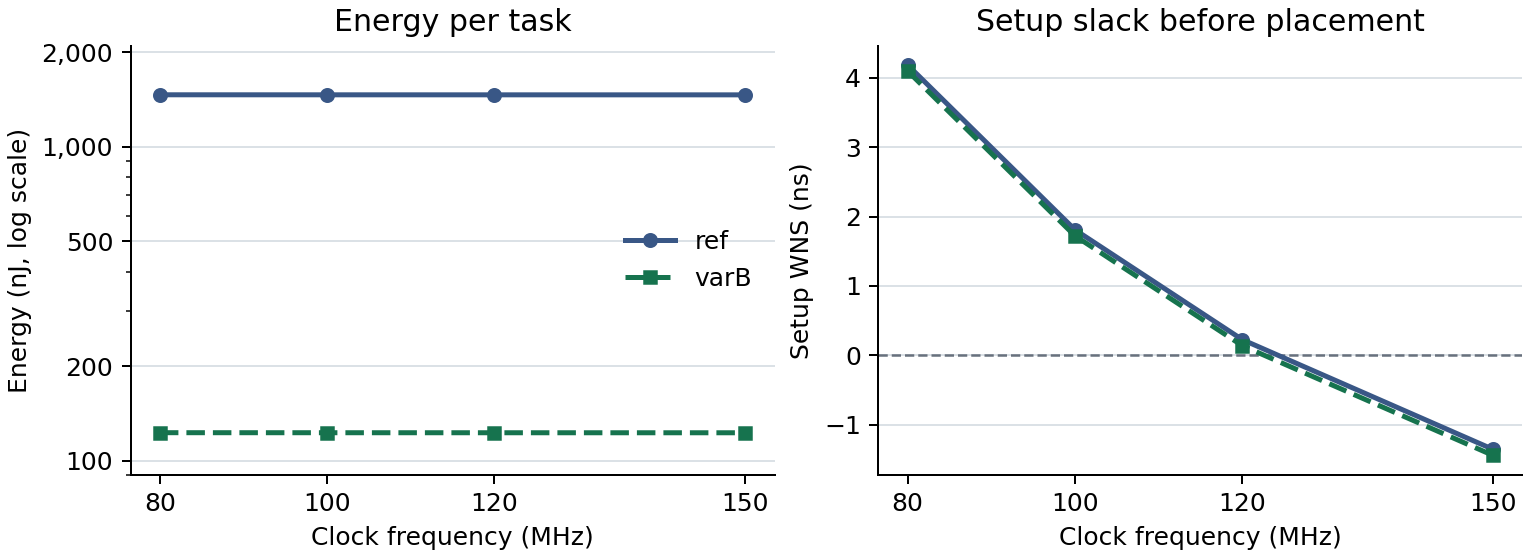
\includegraphics[width=\linewidth]{figures/p4-frequency-sweep.png}
\end{center}
\footnotesize
各方案复用 100 MHz 映射网表。TT 1.10 V 下重放同一随机任务，80 至 150 MHz 的
单任务能耗变化小于 0.06\%。\par\smallskip
120 MHz 时布局前 setup WNS 为 +0.226 ns（ref）与 +0.139 ns（varB）。
150 MHz 两者均小于零。主对照采用 100 MHz。
\end{frame}

\begin{frame}[t]
\frametitle{\textbf{布局布线阶段结果}}
\footnotesize
\begin{center}
\begin{tabular}{lrr}
  \toprule
  100 MHz，Innovus 25.12 & ref & varB \\
  \midrule
  布线后单元面积（$\mu$m$^2$） & 待提取 & 75\,162.024 \\
  芯片占地（$\mu$m$^2$） & 待提取 & 130\,767.437 \\
  SS setup WNS（ns） & 待提取 & $-0.875$ \\
  FF hold WNS（ns） & 待提取 & $-0.421$ \\
  NanoRoute DRC 标记 & 待核对 & 115\,649 \\
  连通性检查 & 待核对 & 通过 \\
  \bottomrule
\end{tabular}
\end{center}
\begin{block}{后端进度}
  两套 100 MHz TT 网表采用相同的 SMIC 40LL 工艺库和布线设置。
  ref 已完成 CTS，正在从检查点续跑详细布线。
  varB 仍有时序与几何违例。
\end{block}
\end{frame}

%%%% ============ 6 结论 ============
\section[结论]{结论}

\begin{frame}[t]
\frametitle{\textbf{位宽、行缓冲和并行度的取舍}}
\footnotesize
\begin{center}
\fitbox{%
\begin{tabular}{llll}
  \toprule
  维度 & 做法 & 拿到什么 & 付了什么 \\
  \midrule
  精度 & 16 $\to$ 10 bit & 乘法器面积降到 39\% & RMSE 仍留 24 倍余量 \\
  面积 & 全矩阵 $\to$ 行融合 & 面积 $2.07\times$ & 双缓冲及流水控制 \\
  时延 & 1 $\to$ 4 lane & 周期 $2.88\times$ & 4 个乘法器，面积 $1.14\times$ \\
  能耗 & 以上叠加 & $E_0/E=11.92$ & 取决于前三条组合 \\
  \bottomrule
\end{tabular}}
\end{center}
\vspace{1mm}
\begin{columns}[t,onlytextwidth]
  \column{.50\textwidth}
  \scriptsize
  \textbf{数值与结构选择}
  \begin{itemize}
    \item 输入区间固定，Q/K/V 统一采用定点量化。
    \item 四路乘加缩短点积周期，行融合缩小中间存储。
    \item \texttt{fold\_l2e} 面积收益为 1.27\%，同时增大定点误差。
  \end{itemize}
  \column{.47\textwidth}
  \scriptsize
  \textbf{实验条件}
  \begin{itemize}
    \item 以仓库当前 ref 为基线，最终方案选 varB。
    \item 综合和任务窗口功耗使用 TT/100 MHz。
    \item 后端按 SS 检查 setup，按 FF 检查 hold。
  \end{itemize}
\end{columns}
\end{frame}

\begin{frame}[t]
\frametitle{\textbf{结论}}
\footnotesize
\begin{enumerate}
  \item \textbf{数值验证。}\;
  10 bit 定点 $+$ 16 项 LUT 的 $2^{-f}$ $+$ 每行一次倒数：RMSE 0.0025（限 0.06，24 倍余量）、
  MaxAE 0.0060（限 0.20，33 倍余量），乘法器面积降到 16 bit 方案的 39\%。

  \item \textbf{行融合。}\;
  $S/P$ 采用 16 深行缓冲，取消两张整矩阵存储。
  最终 varB 相对 ref 的面积改善 $2.36\times$、能耗改善 $11.92\times$。

  \item \textbf{缓冲释放时机。}\;
  归一化后释放指数行缓冲，单变量对照节省 315 拍。
  同一随机任务能耗降低 11.5\%，两版逐位结果一致。
\end{enumerate}
\vspace{1mm}
\begin{block}{\textbf{\scriptsize 测量范围}}
  \scriptsize
  门级任务功耗基于零延迟波形。配对后端实验单独报告 RC 提取、时序和几何检查结果。
\end{block}
\end{frame}

%%%% ============ 致谢 ============
\section*{}
\begin{frame}
\begin{center}
  \begin{minipage}{1\textwidth}
    \centering
    \setbeamercolor{mybox}{fg=white, bg=black!60!green}
    \begin{beamercolorbox}[wd=0.72\textwidth, rounded=true, shadow=true]{mybox}
      \LARGE \centering 谢谢，请提问
    \end{beamercolorbox}
  \end{minipage}
\end{center}
\vspace{5mm}
\begin{center}
  \footnotesize
  汪涵 \; 266900 \quad$\cdot$\quad 黄昌文 \; 266909 \quad$\cdot$\quad 许心怡 \; 269873 \quad$\cdot$\quad 郭丰硕 \; 266617
\end{center}
\vspace{4mm}
\begin{center}
  \scriptsize
  东南大学 \; 集成电路学院 \; · \; 数字集成电路设计 2026 秋 \; · \; 题目一
\end{center}
\end{frame}

\end{document}
